\documentclass{article}

\usepackage{graphicx}

\title{Develop a Better Understanding of the Factors Involved With Facilitating the Movement of Refugees From Their Countries of Origin Into Safe Haven Countries}
\author{Jacob Denson}

\begin{document}

\maketitle

This problem breaks down into multiple problems.

\begin{enumerate}
    \item {\bf What are the factors involved with moving refugees?}

    What attributes enable or inhibit the safe and efficient movement of refugees. As an example, the individuals (plus resources the individuals have), routes, types of transportation, country capacity (plus entry points). The UN asks us to prioritize the health and safety of refugees.

    Total numbers of refugees in the system and at each node, entry points for refugees, possible routes, popularity and capacity of those routes, length of routes, infrastructure for accommodation along routes, and capacity for receipt of refugees.

    Safety will be optimized by minimizing the risk that any individual may not complete a route. We define a measure of risk that incorporates information about liklihood of illness, death (i.e. drowning on water routes), and other dangers of travel that may be exacerbated for routes with high throughput for a given route. 

    We choose a monotonically increasing density function that models the risk of not completing the route. Higher population densities along a route result in a higher risk than lower densities. We assume that low densities have low risk and that high densities have high risk, so density may have an exponential, sigmoidal or linear relationship to risk. If we assume that once a threshold density is reached, risk increases at a slower rate then, a sigmoidal curve may approximate the relationship between density and risk more accurately than an exponential or linear relationshp. However, since we have decided to use a linear programming model  If data becomes available, then a more realistic density-risk function may be substituted into the model.

    Calculation of risk must also relate the length of the route to the density, perhaps with a linear relationship. 

    Efficiency - With high numbers of migrants, where do bottlenecks occur? Why do bottlenecks occur, and  What measure may be used to evaluate the efficiency of a system? Penalty for slower travel and for long waits in camps before reaching the end destination and exiting the system. Policy that prevents a high number of individuals existing without citizenship to a country should be preferred.

    Assumptions: All migrants who make it to their destination travel at the average rate. Due to our choice of a linear programming model, all relationships are linear. 

    \item {\bf How do we gain a better understanding of the factors?}

    Create a model of optimal refugee movement, considering accessibility of transport, safety of route, and resource capacities of countries. Use metrics considered to predict the number of refugees that are to be moved, as well as the rate and point of entry necessary to accomodate their movement. Explain new elements you have incorporated into the migration process.

    It should be noted that we must account for dynamically changing environmental factors. Our model should exhibit a use of endogenous change (prepositioning and allocating resources) to form the best route planning approach. Exogenous parameters (unavoidable, unpredictable events, like the terrorist attack in France) must also be considered.

    Graph with connected nodes. Known number of people at a number of entry points. Need to optimize distribution.

    Modelling methods considered:
    Stochastic Differential Equations are used in the stock market because individual factors cannot be influenced. This may be a way to realistically model the randomness of individual refugee movement. However, this type of model is difficult to optimize, which may make it difficult to meet our objective to optimize refugee movement. The use of stochastic programming may allow for optimization of the model. Stochastic effects are generally more important when you are dealing with small population sizes\footnote{Vries {\em et al.} 2006}. Since stochastic effects will likely have little impact on the overall movement of large groups of refugees along major migration routes, it is reasonable to model this situation using deterministic models. 

    Propogater models

    Modelling refugee movement may be treated as a social network problem, with multiple sources and sinks. Travel through the system may be described using fluid dynamics with partial differential equations describing each time step. One way to model exogenous events would be to 

    Create a graph where edges describe travel routes and vertices represent various locations that refugees may travel through and to.

    What do we know about our system?
    How much feedback exists in our system? Is it a closed system? 
    Let us consider a model that describes refugees that are not settled. This includes migrants who are residing in refugee camps in Northern Africa, migrants who are in transit, and migrants who have reached a destination, but do not have accepted migrant status (?) and have not been officially settled in the country. If a migrant becomes officialty settled then they have left the system. 

    Starting with a basic model, each possible country near Europe where there may be a substantial refugee population is represented as a vertex on a graph. The edges between vertices represent the connectivity between locations for refugees. Connectivity may be described by an adjacency matrix that contains information about travel adjacencies, i.e. which countries are connected to others by travel routes. Then, this information can be interpreted to generate paths. Rates of travel along edges may vary based on qualities of the travel route including capacity, distance, modes of transportation available and risk to migrants. Once these variables and parameters are related on a graph, we need to learn about the dynamics of the system.

    One way to inform the movement of refugees from their country of origin into safe haven countries is to learn about how our system behaves when safety and efficiency are optimized. Safety and efficiency are optimized when risk is minimized and \underline{\ \ \ \ }, respectively. Risk and \underline{\ \ \ \ } can be combined linearly, resulting in an overall measure that determines We chose to use linear programming to optimize our system because it can always be solved. D

    Question?

    \item {\bf Propose a set of policies to the UN}

    Write a report to the UN, proposing a set of policies to enact which will support the conditions for optimal migration (optimal to the UN's views).
\end{enumerate}

The 1951 refugee convention defines a refugee to be ``owing to a well-founded fear of being persecuted for reasons of race, religion, nationality, membership of a particular social group or political opinion, is outside the country of his nationality, and is unable to, or owing to such fear, is unwilling to avail himself of the protection of that country''\footnote{http://www.unhcr.org/pages/49da0e466.html}, rather than a migrant, who is just someone moving from one country to another.

Immigrants travel multiple routes -- beginning at the middle east, and travelling through the West, East, and Central Mediterranean, the West Balkans, the Eastern Borders, and from Albania to Greece.

\begin{center}
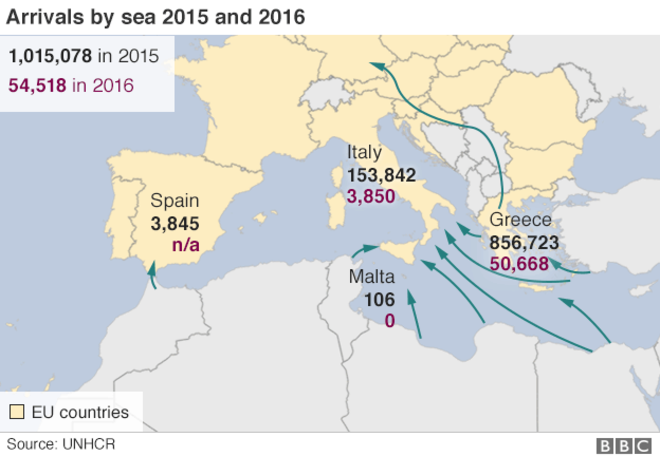
\includegraphics[scale=0.5]{travelmap}
\end{center}

\begin{enumerate}
    \item The majority of refugees resettle in the middle eastern countries of Jordan, Lebanon, and Turkey.
    \item 1,015,078 refugees arrived by sea in 2015.
    \item 942,000 refugees sought asylum in the European Union in 2015\footnote{Eurostat}.
    \item 315,000 have sought asylum in Germany, yet more than 1 million have been counted in Germany's EASY system\footnote{http://www.bbc.com/news/world-europe-34131911}.
    \item 174,055 applied in Hungary.
\end{enumerate}

Illegal immigration is dangerous, both for political relationships ensuring sustained immigration, and the danger to the immigrants of crossing the border.

\begin{enumerate}
    \item Poorly managed camps in Hungary damaged migrants reputation, leading to a surge in the popularity of the radical nationalist Jobbik party\footnote{http://www.bbc.com/news/world-europe-34280460}. It is difficult to control the way countries will handle the immigration crises, so this is an exogenous factor.
    \item In other countries, such as Germany, strong moral foundations protect the influx of immigration\footnote{http://www.bbc.com/news/world-europe-33700624}, with little (and strongly opposed) backlash at the new immigration policies.
    \item The Paris attacks threatened relations about refugees. A Polish minister stated that ``we were too idealistic'' \footnote{http://www.bbc.com/news/world-europe-34826438}. The attack deepened the level of insecurity across Europe, since it was believed that the terrorists snuck into the country with refugees. Regardless of the truth of these facts (the leader was Belgian), the coinciding events were treated as such, and has lead to border problems in the country.
\end{enumerate}

The difference in each country's utility to hold refugees is integral to how important it is to uphold their immigration policy.

Economically, immigration should be beneficial to host countries. A well defined immigration policy, distributed across the continent, should not be a problem

\begin{enumerate}
    \item Our best evidence suggests that immigration is usually economically beneficial for host countries. The majority of refugees arriving on European shores are able-bodied and unlikely to be an exception to this general rule. So the best way for Europe to help would be to offer immediate legal residency and access to labour markets. It might be politically expedient to restrict access to some welfare benefits but most migrants will be keen to work regardless\footnote{http://www.telegraph.co.uk/news/worldnews/europe/11845205/Why-do-refugees-and-migrants-come-to-Europe-and-what-must-be-done-to-ease-the-crisis.html}.
\end{enumerate}

Note that our proposal is a short term proposal. The only way to permanantly ease the migrant situation in Europe is to end the conflicts that make people flee their countries in the first place. Therefore, we should only project our models into short time periods in the future (5 years?).

How much do refugees move once they enter countries? Evidence to suggest immigrants attempt to flee Hungary and enter Germany.

Things to research for tomorrow:
\begin{enumerate}
    \item History, pertaining to dangers and effects of certain decisions on immigration policy.
    \item The UN's framework and objectives for the goals of refugee immigration.
    \item How NGOs fit into the immigration picture.
    \item How much does immigration cost?

    \item Look up the application for official refugee status.

    Look in paper\footnote{$http://fra.europa.eu/sites/default/files/fra-focus_02-2015_legal-entry-to-the-eu.pdf$} and also \footnote{$https://www.hrw.org/report/2015/11/16/europes-refugee-crisis/agenda-action$}.

    The first step for a refugee is to arrive and register in a UNHCR refugee camp outside of Syria. The UNHCR then refers those who pass the first stage of vetting to the U.S. government refugee process (as described above). The National Counterterrorism Center, the Terrorist Screening Center, the Department of Defense, the FBI, Department of Homeland Security, and the State Department use biometrics and biographical information gleaned through several interviews of the refugee and third-party persons who know him or could know him to make sure applicants really are who they claim to be, to evaluate their security risk, and to investigate whether they are suspected of criminal activity or terrorism.  Numerous medical checks are also performed.  During this entire screening process, which takes about three years for Syrians, the refugee has to wait in the camp. If there is any evidence that the refugee is a security threat, he or she is not allowed to come to the United States\footnote{http://www.cato.org/blog/syrian-refugees-dont-pose-serious-security-threat}.

    \item How many immigrants do we need to accomodate?

    3 Million refugees to enter the EU by the end of 2016\footnote{http://www.independent.co.uk/news/world/europe/eu-expecting-another-3-million-refugees-migrants-before-end-of-2016-a6722096.html}.

    \item What Routes do immigrants take - what type of transportation are they taking?

    \item Where are immigrants trying to go?
    \item Quotas for countries.
    \item Legal routes for immigrants immigrate.
\end{enumerate}

$http://www.pewresearch.org/fact-tank/2015/04/24/refugees-stream-into-europe-where-they-are-not-welcomed-with-open-arms/ft_15-04-22_eu-immigration/$



\begin{center}
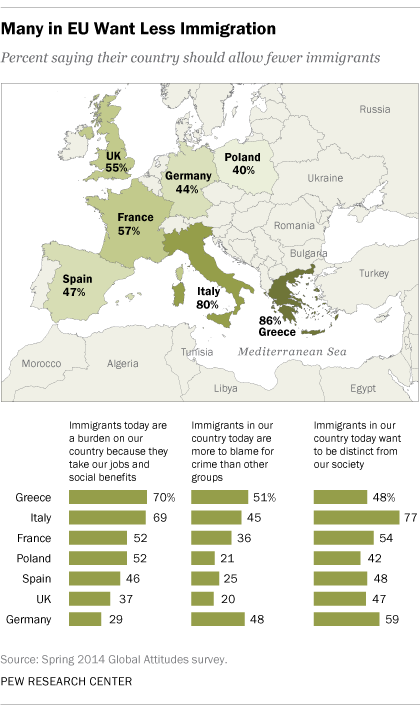
\includegraphics[scale=0.5]{ImmigrationPoll}
\end{center}

\end{document}